\chapter{La collecte et la transmission de données}

\section{Communication Wifi}

Un des points qui peu être amélioré dans notre projet est le système de transmission de données. Nous avions opté pour une transmission GSM/3G en supposant que la localisation des ruchers ne pouvaient pas être couverte par un réseau Wifi. Cela obligera donc l'apiculteur à se procurer une carte SIM chez un opérateur téléphonique. Or, ce mode peut devenir couteux sur plusieurs de ses ruches sont équipés de notre cadre. C'est pour cela qu'il peut être intéressant de développer un système de communication Wifi en plus de celle GSM/3G en fonction du lieu des ruches. Nous avons commencé à développer ce type de transmission avec les modules Wifi présents au club robotique de l'ENSTA Bretagne en se reposant sur le protocole HTTP.   

\begin{figure}[h!]
\centering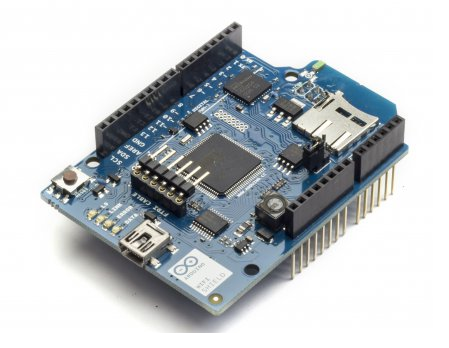
\includegraphics[trim= 0cm 0cm 0cm 0cm,scale=0.65]{wifi.png}
\caption{\label{fig:wifi} Shield Wifi Arduino}
\end{figure}

\clearpage

\section{Traitement du son}

Le cadre de mesure possède bien un capteur de son permettant de recueillir le bruit ambiant et renseigner l'apiculteur sur la présence d'abeilles et l'activité de sa ruche. Néanmoins, l'état de l'art mené nous a permis de connaitre la fréquence émise par les ouvrières avant un essaimage. L'idée est de pouvoir effectuer un traitement du signal sonore reçu et repérer la fréquence d'essaimage. Nous avons essayer de repérer des fréquences "pures" générées en utilisant Audacity et Matlab pour tester les capacités de notre capteur avec succès bien malgré un bruit important.
Pour cela, deux solutions sont envisageables: \\

\indent - Télécharger la bibliothèque FFT d'Arduino présente sur GitHub. \\
\indent - Prévoir un programme de traitement du son sur le serveur. \\

Dans les deux cas, nous avons aussi envisagé un filtre physique placé à la sortie du capteur de son afin d'avoir un meilleur filtrage en amont.

\begin{figure}[h!]
\centering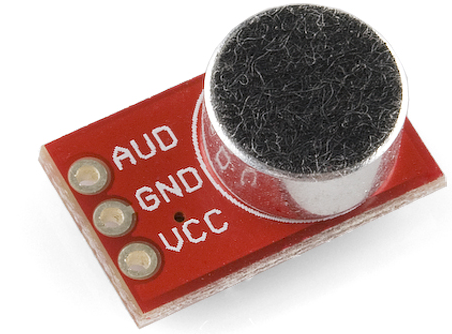
\includegraphics[trim= 0cm 0cm 0cm 0cm,scale=0.5]{son.png}
\caption{\label{fig:son} Capteur de son présent dans le cadre de mesure}
\end{figure}

\section{Alimentation}

Pour l'alimentation, il peut être intéressant de développer un système informant l'apiculteur de l'état des piles/batteries présents dans le boitier avec la carte Arduino. \\
Il pourra aussi être intéressant de développer un système plus écologique comme par exemple une éolienne ou des panneaux solaires que nous disposerons au milieux du rucher et où les différents cadres viendront s'alimenter. Coupler cette solution avec une communication Wifi permettra à l'apiculteur d'utiliser le système de cadre de mesure pour un coup minimal. 

\section{Server}

For the moment, for each new measurement a POST request needs to be made. In the case there are many users with many beehives, there will be many requests being made and that could cause a strain on the server, having an impact on scalability. In the future, it should be possible to send new measurements in batches, one single POST request would send a JSON object containing the values for all sensors to that Arduino. It would also be interesting to create a queue. If there is a connectivity problem, the data will wait and then be sent in a single request once connectivity is restored, causing the data not to have "holes" in its timeline.

Another possible improvement is, when creating a new beehive at the web application, it would already create a set of basic sensors that are most commonly used. This would allow a quicker configuration for a new beekeeper's account. 

It would also be optional if the web application generated a text file that could be incorporated into the Arduino, and the Arduino would read from that file and understand which physical sensor corresponds to which unique database entry, automating a configuration that is, for the moment, manual. 